\chapter{Revisão Bibliográfica}
Neste capitulo serão abordados alguns conceitos e técnicas necessárias para
gerar o mapa de altura proceduralmente, além de apresentar alguns trabalhos
relacionados.

\section{Biomas} %Preciso de mais fontes nesta seção, urgente
Existem mais que um conceito de bioma, um bastante adotado considera bioma como
uma área do espaço geográfico, representada por um tipo uniforme de ambiente, o
mesmo pode ser classificado de acordo com o macroclima, fitofisionomia (formação),
solo e a altitude, os elementos que maus caracterizam os ambientes continentais, 
este é o conceito de \cite{coutinho2006conceito}, usando como base descrições
de \cite{walter1986vegetaccao}.

Porém neste trabalho o conceito de bioma vai ser outro, o resultado deste
vai ser unicamente mapas de altura, então a única característica que é relevante
são as altitudes do solo e seus padrões, descartando dados como tipo da
vegetação e sua distribuição, umidade e entre outros. Então no restante 
do trabalho, quando for usado os termos "característica do bioma", o mesmo vai
se referir a alguma característica de altitude do bioma.

Para fins de restringir o escopo do projeto vamos agrupar os biomas por padrões
de relevo e não por fauna e flora como feito no conceito apresentado acima,
estes biomas serão: cordilheiras (cadeias de montanha), planícies.

\section{Representação das Regiões}
Neste trabalho serão implementadas três maneiras de representar a malha de
regiões, com a intenção de poder analisar diferentes maneiras de representar
a malha do terreno.
\subsection{Malhas de quadrado}

\subsection{Malha triangular}
Na figura a seguir tararara \ref{fig:triangle_strips}
\begin{figure}[H]
    \centering
    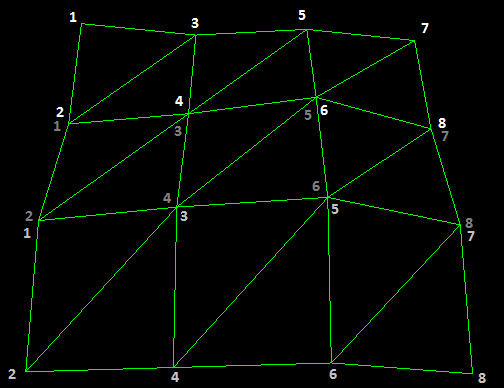
\includegraphics[width=0.7\textwidth]{figuras/triangle_strips.png}
    \caption{Mapa de altura com uma malha de triângulos \cite{trainglestripheightmap}}
    \label{fig:triangle_strips}
\end{figure}
Figura \ref{fig:vbo} xala head xala
\begin{figure}[H]
    \centering
    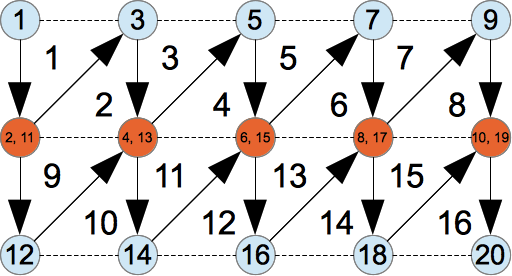
\includegraphics[width=0.7\textwidth]{figuras/vbo.png}
    \caption{Modelo de malhas de triângulos a ser utilizada \cite{androidtrianglestrip}}
    \label{fig:vbo}
\end{figure}


\subsection{Diagrama de voronoi}

\section{Ruído de Perlin}

\section{Mapas de Altura}

\section{Trabalhos Relacionados}

%correção: preciso colocar trabalhos fora deste vínculo e quem sabe adicionar uma seção
%sobre
%Ainda não sei ao certo quais são os trabalhos relacionados que vou apresentar
\subsection{Trabalho de Carli}

\subsection{Bevilaqua}